\section{Assembly reduction with contact and geometric nonlinearity}\label{sec:vf-asm}

\subsection*{Concept and purpose}

\citet{nikiema2026assembly} compare four reduced models for bolted-type assemblies that are preloaded and then loaded further: projection by POD alone, and POD with hyper-reduction by the energy-conserving sampling and weighting method (ECSW), the discrete empirical interpolation method (DEIM) and its unsymmetric variant (UDEIM). The assembly is geometrically nonlinear (total-Lagrangian Saint Venant--Kirchhoff material) and has unilateral contact between its parts. The study rebuilds the 2D benchmark from the text, then generalises the pipeline to 3D (Hex8 and Hex20 elements, an assembly builder, a full-order driver for sequential preloads). The central claims to test are that DEIM and UDEIM fail with plain Newton when the contact force is approximated, that POD and ECSW do not, and that domain partitioning (DP) gives a further saving.

\subsection*{Mathematics as implemented}

The element is total Lagrangian with the Saint Venant--Kirchhoff law: Green--Lagrange strain $\mathbf E=\tfrac12(\mathbf F^{T}\mathbf F-\mathbf I)$, second Piola--Kirchhoff stress $\mathbf S=\lambda\,\mathrm{tr}(\mathbf E)\mathbf I+2\mu\mathbf E$ (plane stress for the 2D element, \anchor{fea_engine.Quad4PlaneStressTL}), internal force $\mathbf f_{\rm int}(\mathbf u)=\int\mathbf B(\mathbf u)^{T}\mathbf S\,\mathrm dV$ and consistent tangent. The reduced model is
\begin{equation}\label{eq:as-pod}
\mathbf u\approx\mathbf V\mathbf q,\qquad\mathbf V^{T}\bigl[\mathbf f_{\rm int}(\mathbf V\mathbf q)+\mathbf f_{\rm c}(\mathbf V\mathbf q)-\mathbf f_{\rm ext}\bigr]=\mathbf 0,
\end{equation}
with $\mathbf V$ the POD of the snapshots at the chosen tolerance $\varepsilon$ on the discarded energy. The hyper-reduced variants replace the projected force by an approximation.

\emph{ECSW} evaluates the projected force on a weighted subset $\mathcal E$ of elements,
\begin{equation}\label{eq:as-ecsw}
\mathbf V^{T}\mathbf f(\mathbf V\mathbf q)\approx\sum_{e\in\mathcal E}\xi_e\,\mathbf V^{T}\mathbf L_e^{T}\mathbf f_e(\mathbf L_e\mathbf V\mathbf q),\qquad\xi_e\ge0,
\end{equation}
with weights from a non-negative least-squares fit to the snapshot force contributions up to a tolerance $\tau$.

\emph{DEIM and UDEIM} approximate the nonlinear force vector by interpolation on a basis $\mathbf\Phi_f$ of force snapshots at selected rows $\mathbf P$,
\begin{equation}\label{eq:as-deim}
\mathbf f\approx\mathbf\Phi_f(\mathbf P^{T}\mathbf\Phi_f)^{-1}\mathbf P^{T}\mathbf f,
\end{equation}
applied to the internal force (DEIM) or to the unassembled element forces (UDEIM); the tangent is approximated in the same way. In the variant added in this study (DEIM-NL, UDEIM-NL) the nonlinear forces include the contact force within the approximated term.

\emph{Domain partitioning.} The package's indicator splits the elements into a part that stays linear and a part that is nonlinear; only the latter is re-assembled in the Newton loop, and only the former is condensed once.

\subsection*{Geometry and mesh: 2D benchmark}

The 2D benchmark is a top-hat strip placed on a flat strip, 100~mm long with a 2.5~mm section, meshed by 324 four-node elements (800 free degrees of freedom); contact acts between the lower face of the top-hat and the flat strip. The parameters \emph{as stated} in the publication leave the upper part far too soft: contact begins in the first load increment, at 0.46~N, whereas the publication has it in the second. \Cref{fig:vf-as-geom} and \Cref{fig:vf-as-mesh} show the geometry and the mesh; \Cref{fig:vf-as-defo} the full-order deformed state.

\begin{figure}[tbp]
\centering
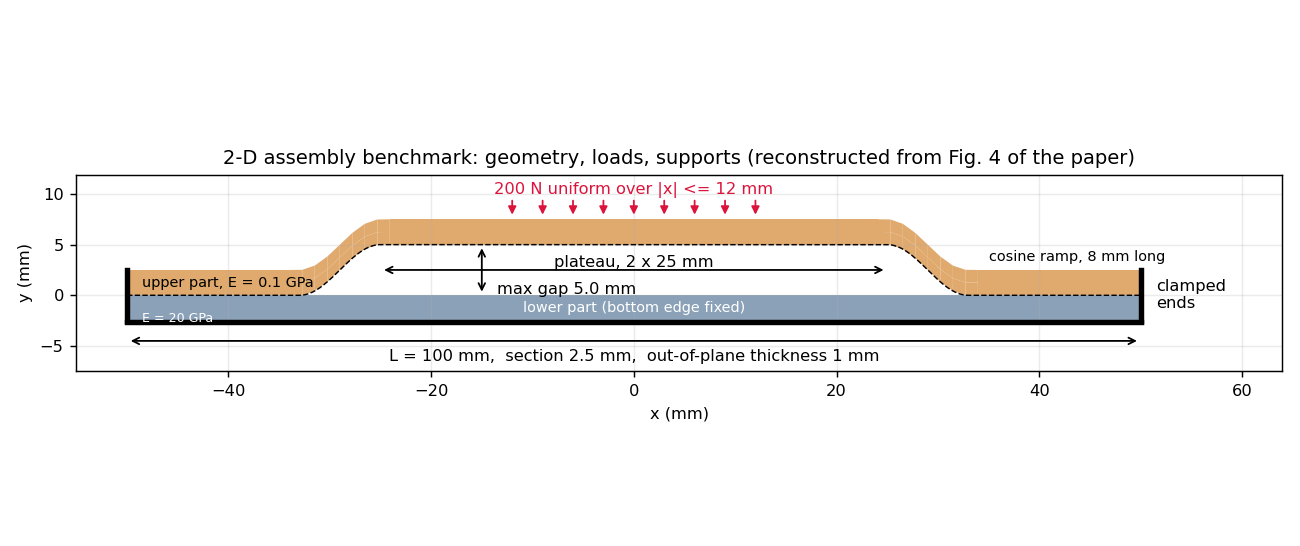
\includegraphics[width=0.95\linewidth]{figures/ch14r/as_geometry.png}
\caption{2D benchmark: the top-hat strip on the flat strip.}\label{fig:vf-as-geom}
\end{figure}

\begin{figure}[tbp]
\centering
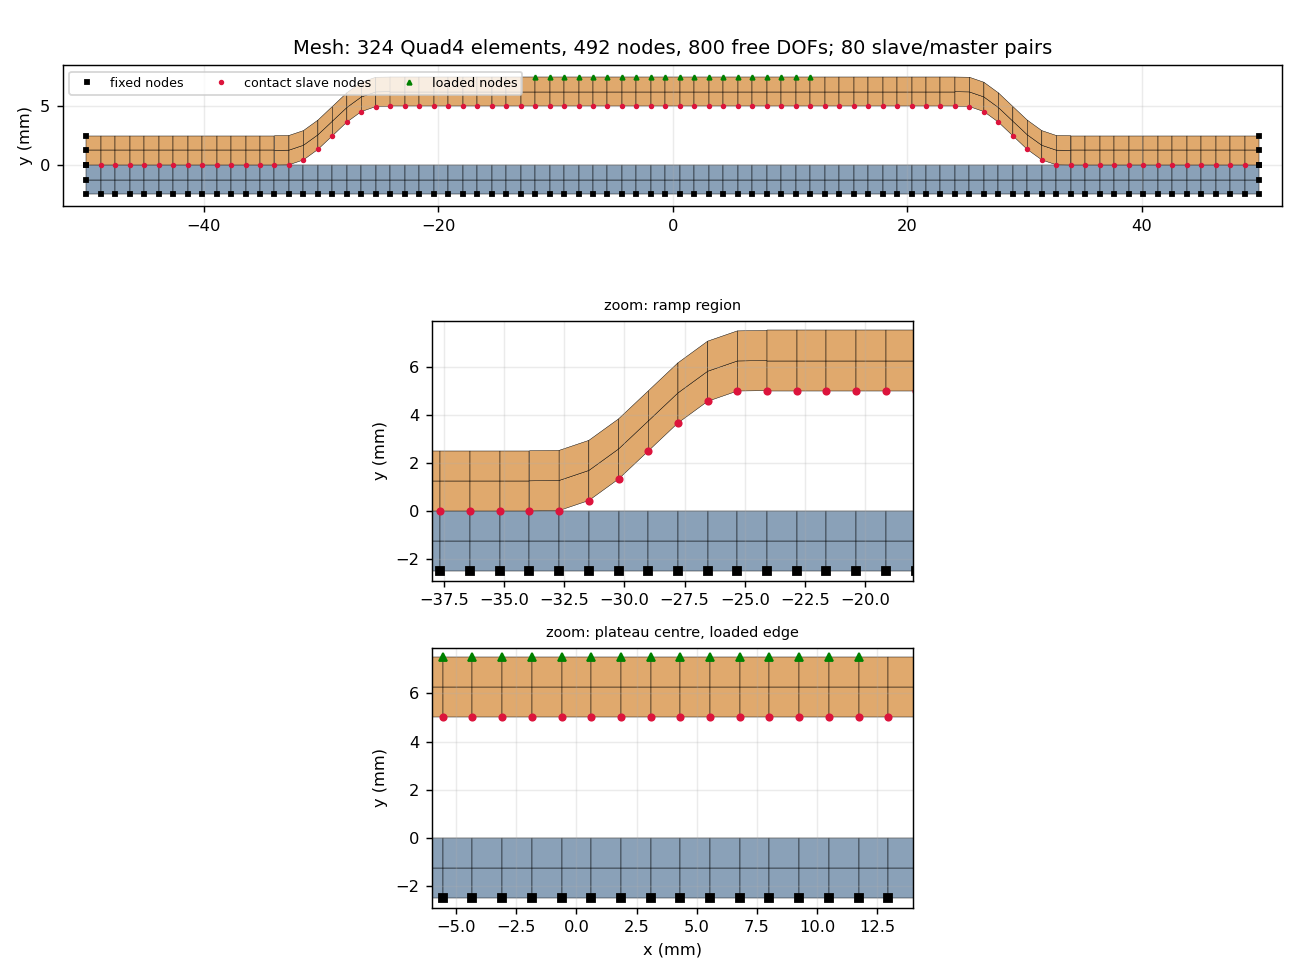
\includegraphics[width=0.95\linewidth]{figures/ch14r/as_mesh.png}
\caption{2D benchmark mesh, 324 elements and 800 free degrees of freedom.}\label{fig:vf-as-mesh}
\end{figure}

\begin{figure}[tbp]
\centering
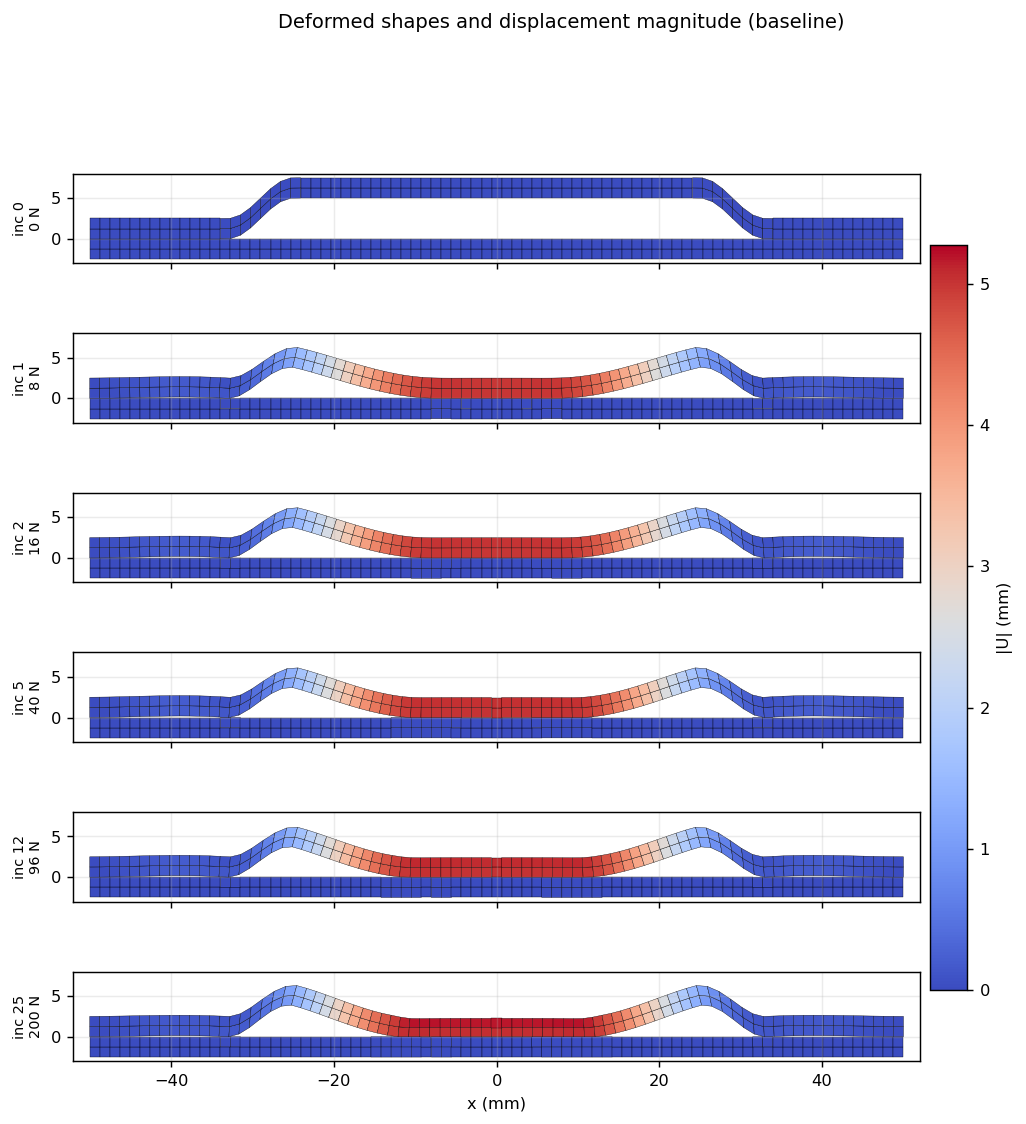
\includegraphics[width=0.95\linewidth]{figures/ch14r/as_baseline_deformed.png}
\caption{Full-order deformed shape of the baseline (as stated) model: contact has already begun in the first increment.}\label{fig:vf-as-defo}
\end{figure}

\subsection*{Results: the 2D benchmark}

\emph{Element and contact onset.} The new element was verified by seven tests. A sensitivity study of 28 variations of the stated parameters (\Cref{fig:vf-as-sens}) shows that the onset of contact is set by the stiffness of the upper part; two single changes, multiplying the Young's modulus of the upper part by 30 or widening the strip to 10~mm, bring the onset into the published window. The study continues with the wider-strip variant, whose singular-value decay is in \Cref{fig:vf-as-svd}. This choice is circumstantial and does not show that the publication used this geometry.

\begin{figure}[tbp]
\centering
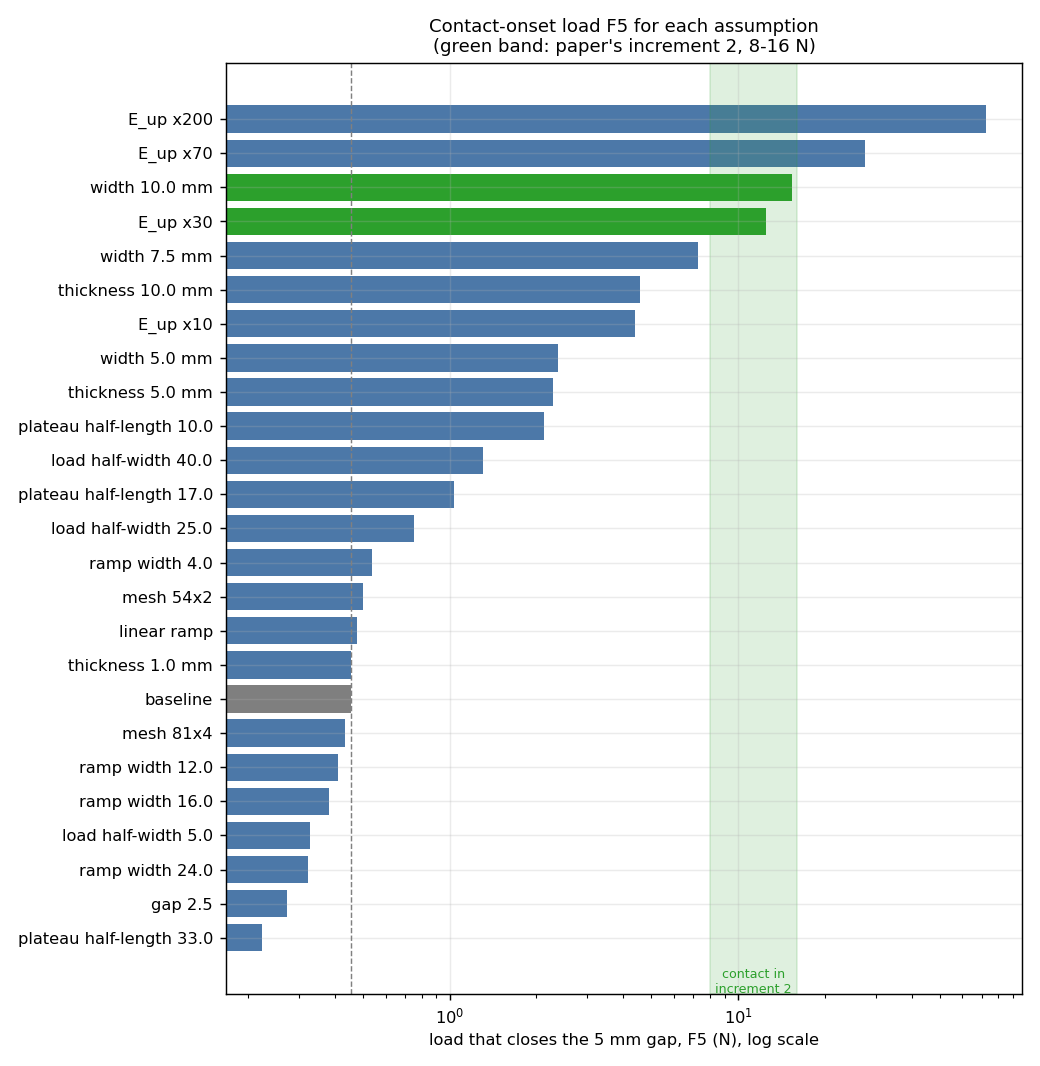
\includegraphics[width=0.85\linewidth]{figures/ch14r/as_sens_bar.png}
\caption{Sensitivity of the contact onset to the 28 parameter variations.}\label{fig:vf-as-sens}
\end{figure}

\begin{figure}[tbp]
\centering
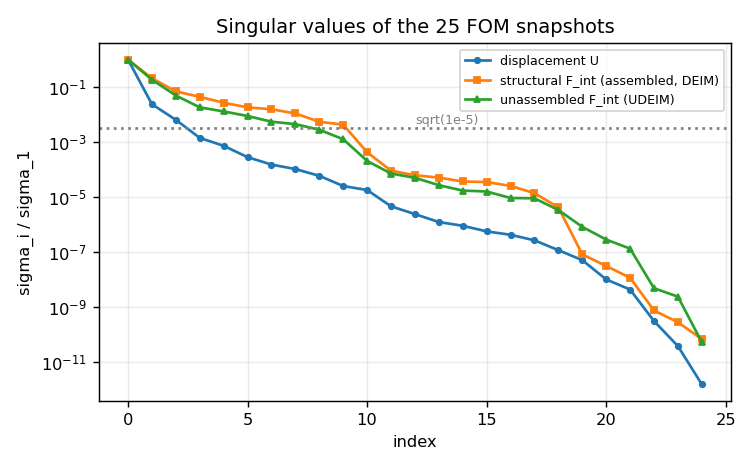
\includegraphics[width=0.8\linewidth]{figures/ch14r/as_width10_svd.png}
\caption{Singular values of the displacement snapshots, 10~mm-wide variant.}\label{fig:vf-as-svd}
\end{figure}

\emph{Plain Newton.} The full-order model needs 86 Newton iterations over the load history (publication 104). The reduced models are in \Cref{tab:vf-as-conv} and \Cref{fig:vf-as-iters}: DEIM and UDEIM fail at $\varepsilon=10^{-6}$ (at increments 2 and 5; publication 18 and 17), POD and ECSW converge, which is the qualitative result of the publication; at $\varepsilon=10^{-9}$ DEIM and UDEIM also converge, which the report could not explain. ECSW was run with $\tau=0.003$ (publication 0.5, which gave no usable model here).

\begin{table}[tbp]
\centering\footnotesize
\caption{2D benchmark with plain Newton (wider-strip variant).}\label{tab:vf-as-conv}
\begin{tabularx}{\linewidth}{@{}>{\raggedright\arraybackslash}p{4.4cm} >{\raggedright\arraybackslash}X >{\raggedright\arraybackslash}X@{}}
\toprule
Quantity & Publication & This work\\
\midrule
Full-order Newton iterations & 104 & 86\\
Failure of DEIM / UDEIM at $\varepsilon=10^{-6}$ & at increments 18 / 17 & at increments 2 / 5; converge at $10^{-9}$\\
POD / DEIM / UDEIM modes & 3 / 11 / 8 & 3 / 10 / 8\\
Error at $\varepsilon=10^{-5}$ & $1.2$--$1.5\,\%$ & $0.94\,\%$\\
Online speed-up POD / DEIM / UDEIM / ECSW & 3.4 / 13.8 / 15.8 / 18.4 & 1.4 / 11.3 / 14.8 / 12.8\\
ECSW tolerance $\tau$ & 0.5 & 0.003\\
\bottomrule
\end{tabularx}
\end{table}

\begin{figure}[tbp]
\centering
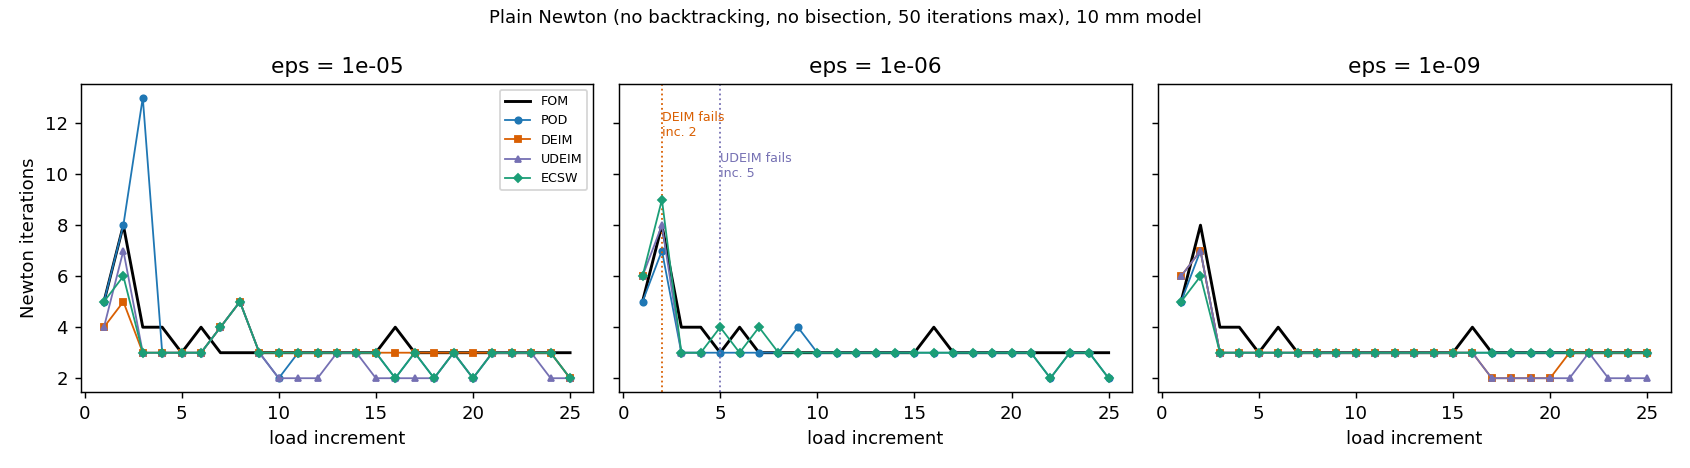
\includegraphics[width=0.85\linewidth]{figures/ch14r/as_rom_iters.png}
\caption{Newton iterations per load increment for the full-order and reduced models.}\label{fig:vf-as-iters}
\end{figure}

\begin{figure}[tbp]
\centering
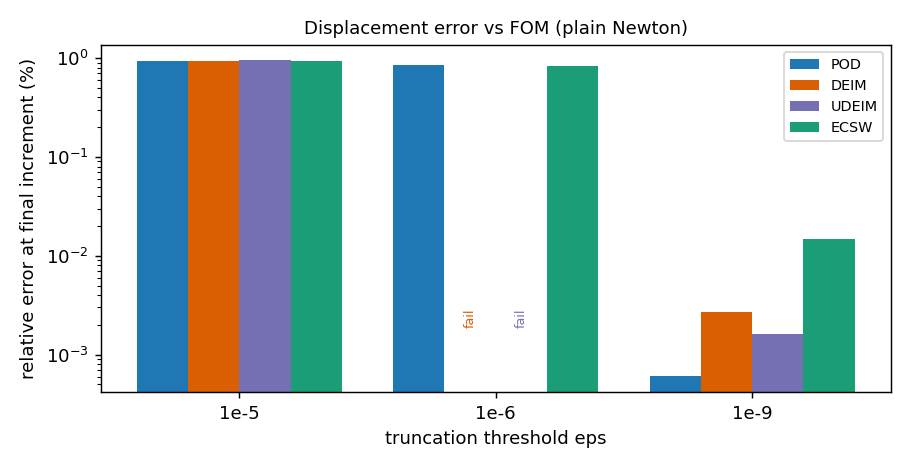
\includegraphics[width=0.85\linewidth]{figures/ch14r/as_rom_errors.png}
\caption{Error of the reduced models against the full-order model at three tolerances.}\label{fig:vf-as-errors}
\end{figure}

\begin{figure}[tbp]
\centering
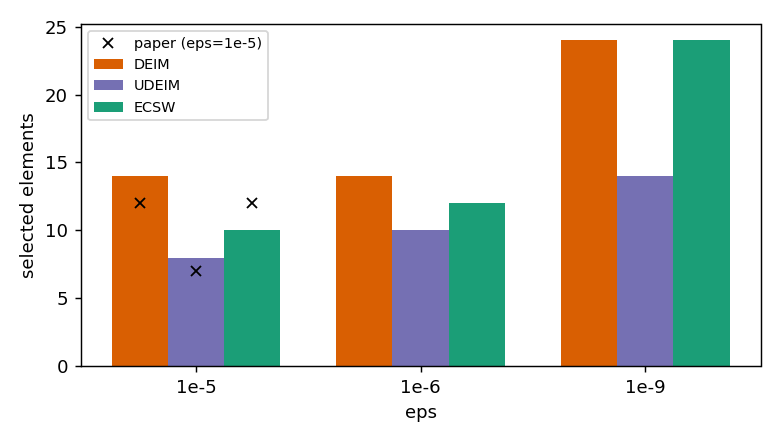
\includegraphics[width=0.85\linewidth]{figures/ch14r/as_rom_elements.png}
\caption{Elements evaluated per iteration against error for the converged runs.}\label{fig:vf-as-elements}
\end{figure}

\begin{figure}[tbp]
\centering
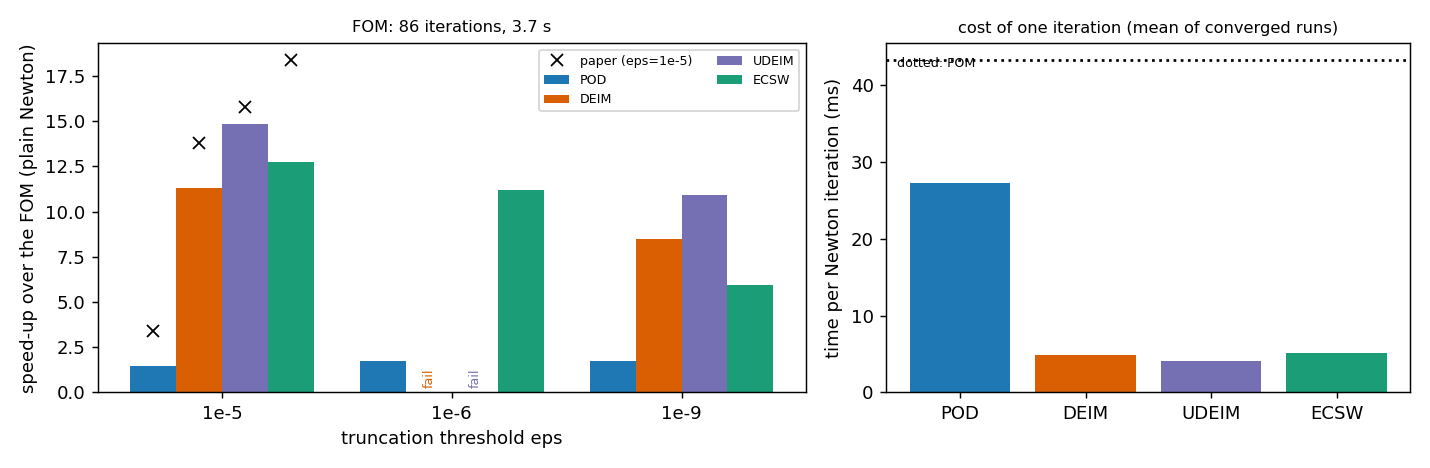
\includegraphics[width=0.85\linewidth]{figures/ch14r/as_timing.png}
\caption{Online timing of the reduced models.}\label{fig:vf-as-timing}
\end{figure}

\begin{figure}[tbp]
\centering
\includegraphics[width=0.95\linewidth]{figures/ch14_asm.pdf}
\caption{2D assembly of \citet{nikiema2026assembly}, plain Newton. (a) Error of the last increment for the four reduced models at three tolerances; crosses mark runs that did not converge (DEIM and UDEIM at $\varepsilon=10^{-6}$). (b) Converged runs: error against the number of elements evaluated per iteration. POD error at $\varepsilon=10^{-5}$: \cvfAsmPodErr.}\label{fig:vf-asm}
\end{figure}

\emph{Domain partitioning.} With the package's indicator at threshold 0.1 the reduced model reproduces the full model to $0.29\,\%$, but 147 to 243 of the 324 elements stay nonlinear, so the speed-up is at most $2.8$ (\Cref{fig:vf-as-dp}, \Cref{fig:vf-as-dptr}). A scan of the number of modes is in \Cref{fig:vf-as-scan}.

\begin{figure}[tbp]
\centering
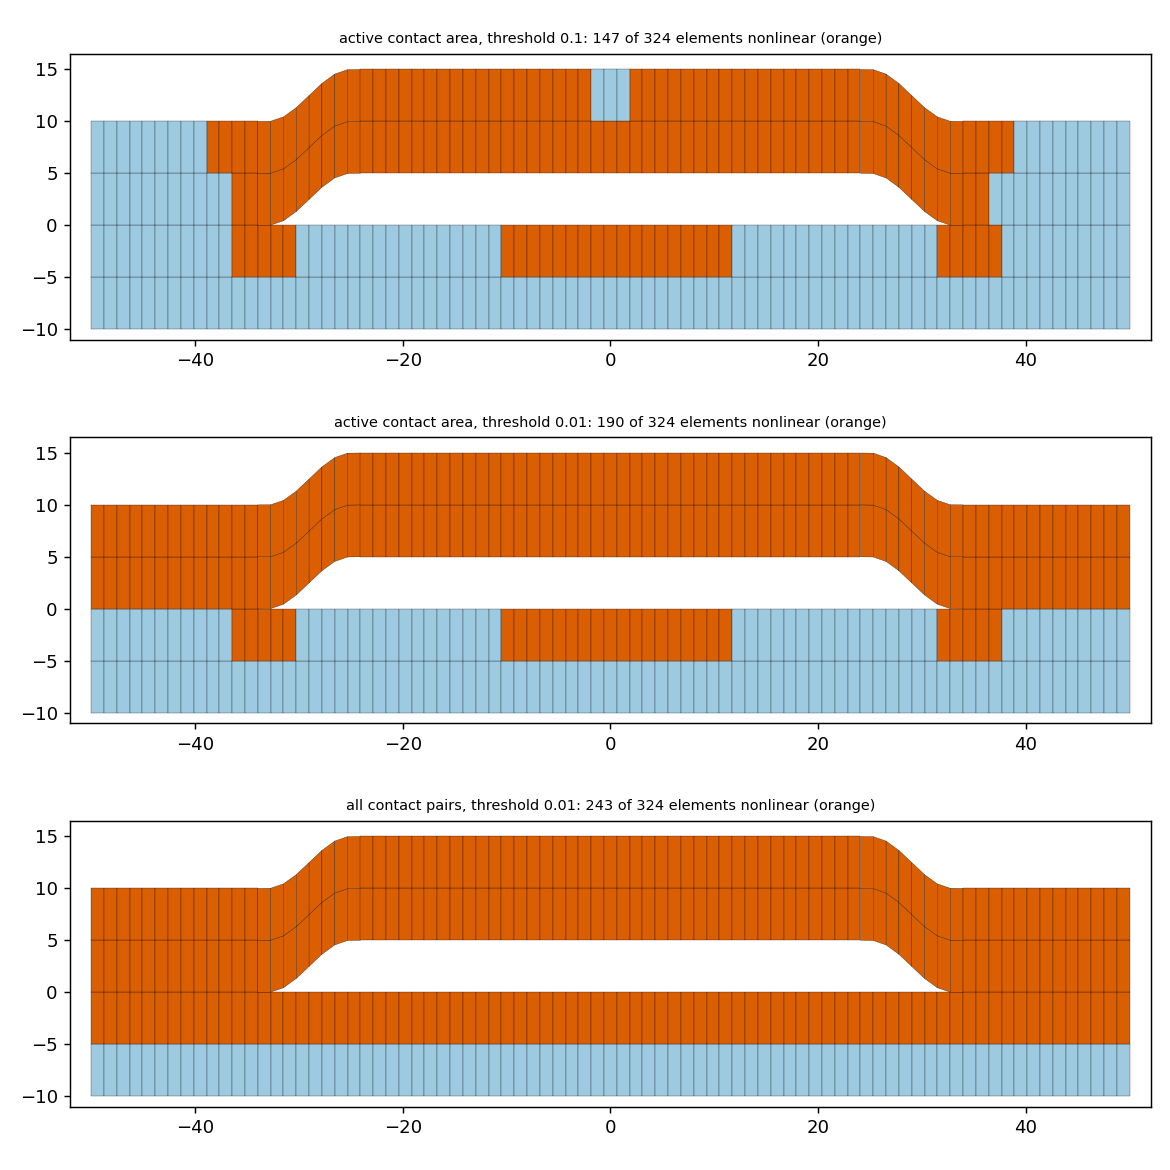
\includegraphics[width=0.85\linewidth]{figures/ch14r/as_dp_zones.png}
\caption{Linear and nonlinear zones from the partitioning indicator.}\label{fig:vf-as-dp}
\end{figure}

\begin{figure}[tbp]
\centering
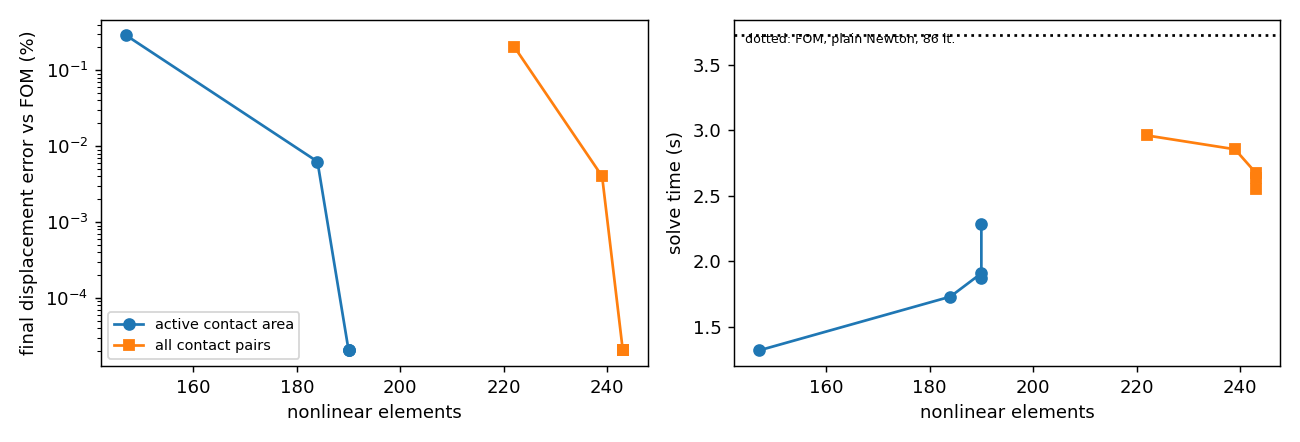
\includegraphics[width=0.85\linewidth]{figures/ch14r/as_dp_tradeoff.png}
\caption{Partitioning: error against speed-up as the threshold varies.}\label{fig:vf-as-dptr}
\end{figure}

\begin{figure}[tbp]
\centering
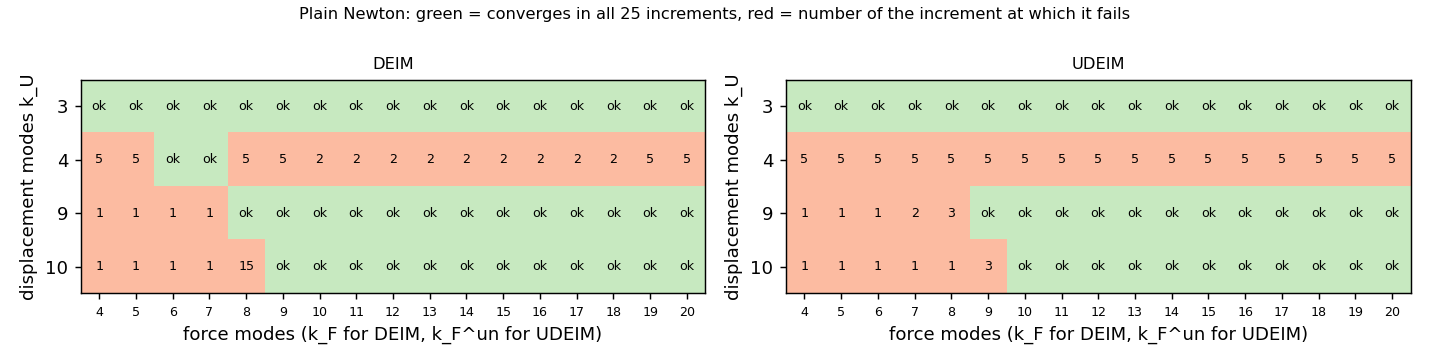
\includegraphics[width=0.85\linewidth]{figures/ch14r/as_mode_scan.png}
\caption{Scan of the number of modes.}\label{fig:vf-as-scan}
\end{figure}

\subsection*{Geometry and mesh: 3D joint}

The 3D pipeline uses total-Lagrangian Hex8 and Hex20 elements (\Cref{fig:vf-as3-el}). Hex8 locks in thin panels, down to $28\,\%$ of the exact bending stiffness, whereas Hex20 gives $0.90$--$0.98$, so Hex20 is used. A scaled butt joint (\Cref{fig:vf-as3-geom}) has 480 Hex20 elements and 12\,087 degrees of freedom. Plain penalty contact made Newton cycle, so a $C^1$-regularised penalty law is used (\Cref{fig:vf-as3-law}); this is a deviation from the publication. The full-order solver uses a symmetric LU factorisation with modified Newton, $3.8\times$ faster than full Newton.

\begin{figure}[tbp]
\centering
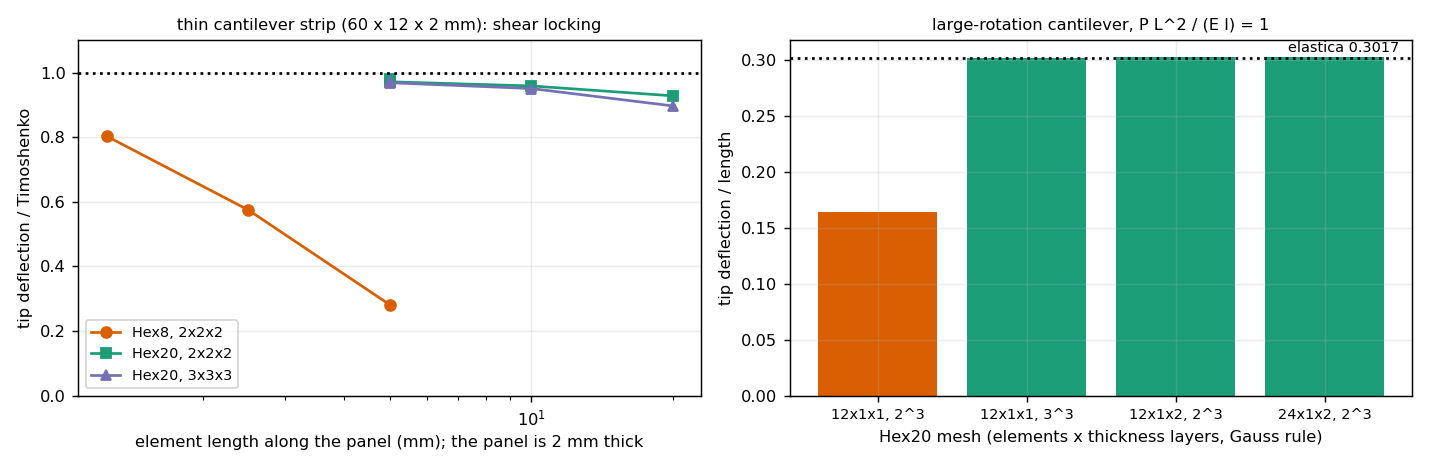
\includegraphics[width=0.7\linewidth]{figures/ch14r/as3_element.png}
\caption{3D elements of the pipeline.}\label{fig:vf-as3-el}
\end{figure}

\begin{figure}[tbp]
\centering
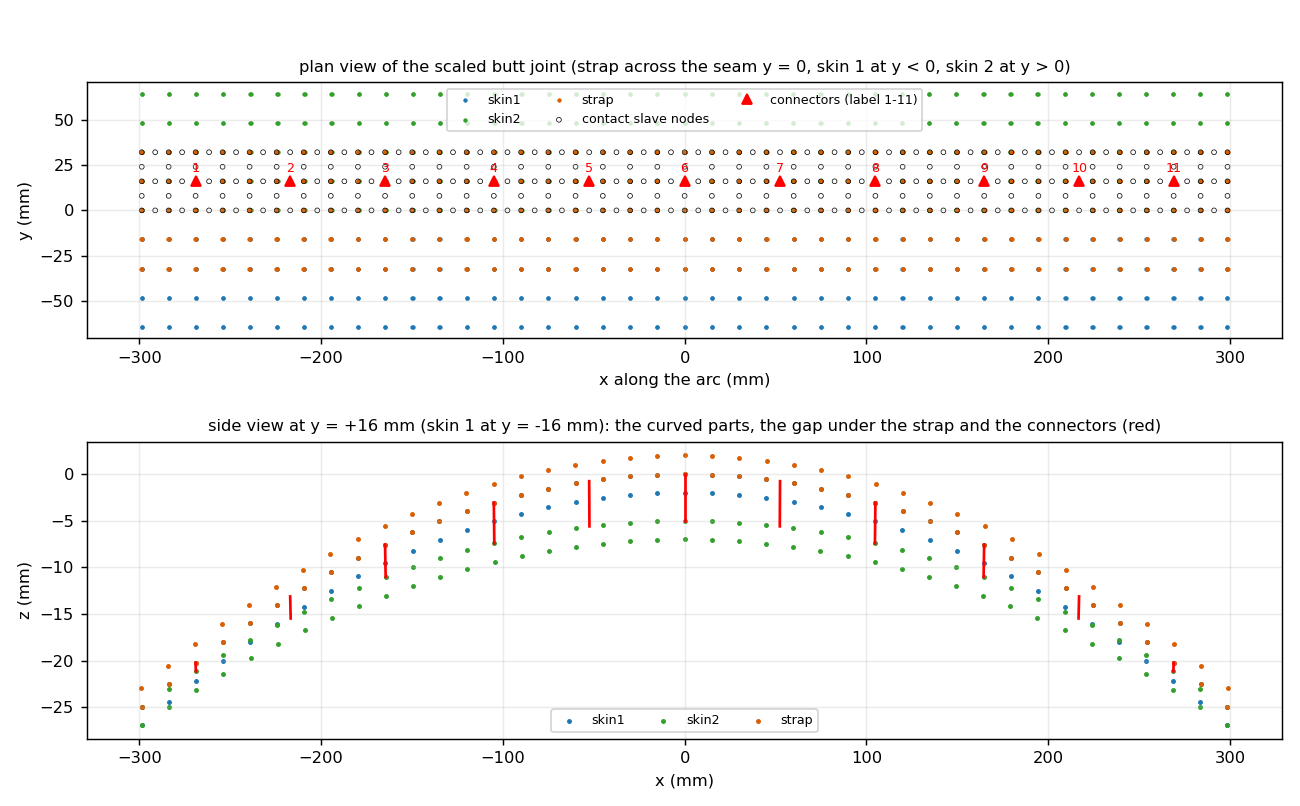
\includegraphics[width=0.95\linewidth]{figures/ch14r/as3_geometry.png}
\caption{Scaled butt joint, 480 Hex20 elements, 12\,087 degrees of freedom.}\label{fig:vf-as3-geom}
\end{figure}

\begin{figure}[tbp]
\centering
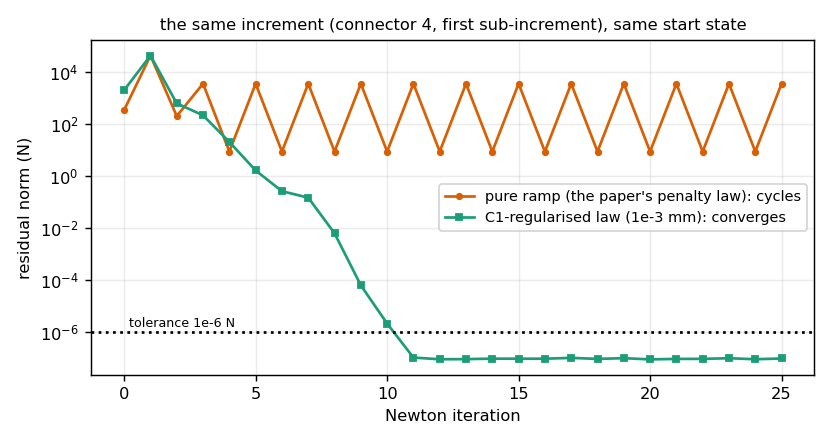
\includegraphics[width=0.7\linewidth]{figures/ch14r/as3_contact_law.png}
\caption{Regularised penalty contact law.}\label{fig:vf-as3-law}
\end{figure}

\subsection*{Results: 3D joint}

With the connectors modelled as rigid (no springs) the nine preload cases of the publication end within $0.3\,\%$ of each other, because the connectors close and the contact absorbs the extra preload, so the benchmark was changed to spring connectors of $k=500$~N/mm, after which the response depends on the preload by $48\,\%$ (\Cref{fig:vf-as3-fom}); the full-order run takes 62~s at 1500~N. \Cref{tab:vf-as3} and \Cref{fig:vf-as3-acc,fig:vf-as3-speed} give the reduced models over nine preloads and four tolerances: POD and ECSW converge in all 36 runs; DEIM and UDEIM as published fail in 34 of 36, because their force approximation is good on training states ($1$--$2\,\%$) and wrong by $10$--$150\,\%$ a short distance off them. The variant that approximates the nonlinear forces including contact (DEIM-NL, UDEIM-NL, an addition of this study, not in the publication) converges in all 36.

\begin{table}[tbp]
\centering\footnotesize
\caption{3D joint with springs: POD error and modes, and speed-up at 1500~N.}\label{tab:vf-as3}
\begin{tabular}{@{}lrrr@{}}
\toprule
 & $\varepsilon=10^{-5}$ & $10^{-6}$ & $10^{-9}$\\
\midrule
POD error (\%) & 1.705 & 0.649 & 0.019\\
POD modes & 20 & 26 & 71\\
Speed-up POD & 1.5 & 1.3 & 1.0\\
Speed-up DEIM-NL & 11.0 & 6.9 & 3.4\\
Speed-up UDEIM-NL & 16.9 & 10.8 & 5.5\\
Speed-up ECSW & 8.8 & 4.3 & 1.4\\
\bottomrule
\end{tabular}
\end{table}

\begin{figure}[tbp]
\centering
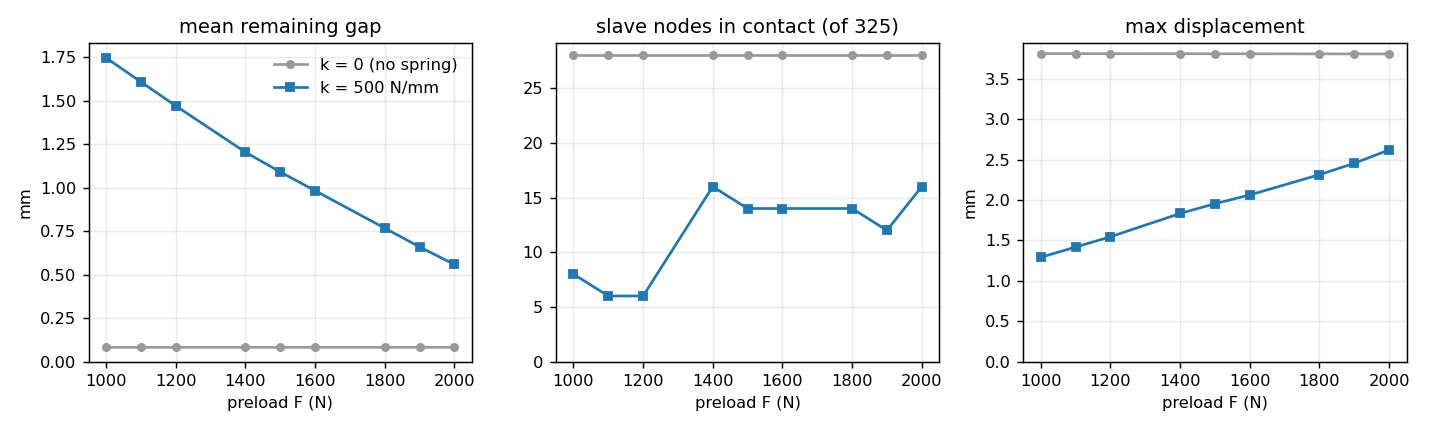
\includegraphics[width=0.85\linewidth]{figures/ch14r/as3_k500_fom.png}
\caption{Full-order response of the spring-connected joint over the nine preloads.}\label{fig:vf-as3-fom}
\end{figure}

\begin{figure}[tbp]
\centering
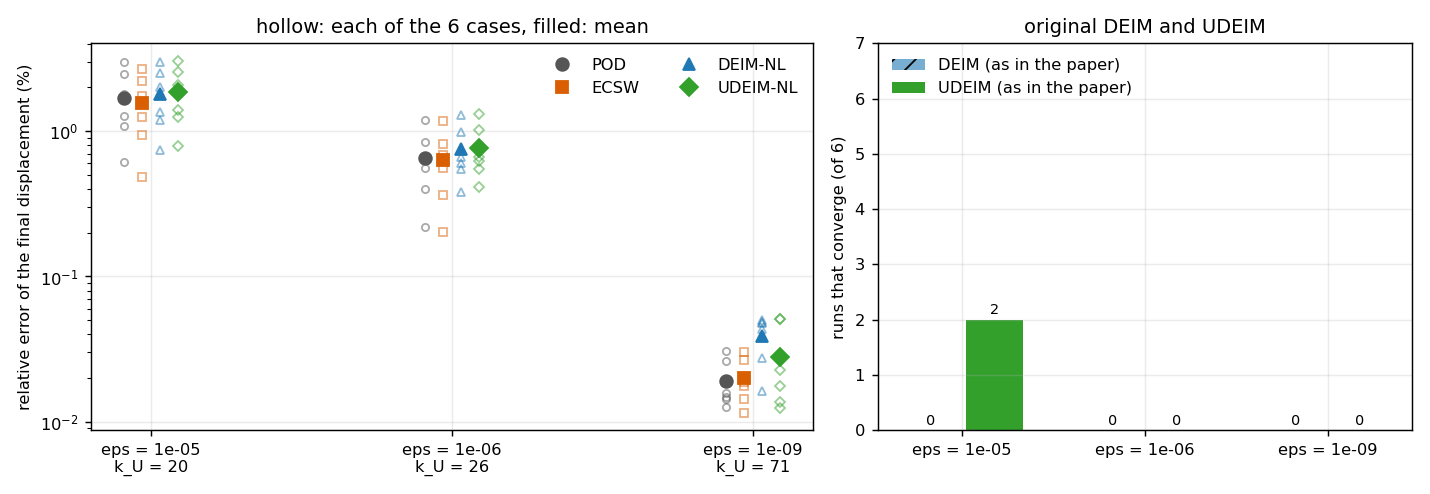
\includegraphics[width=0.85\linewidth]{figures/ch14r/as3_rom_accuracy.png}
\caption{3D joint: accuracy of the reduced models.}\label{fig:vf-as3-acc}
\end{figure}

\begin{figure}[tbp]
\centering
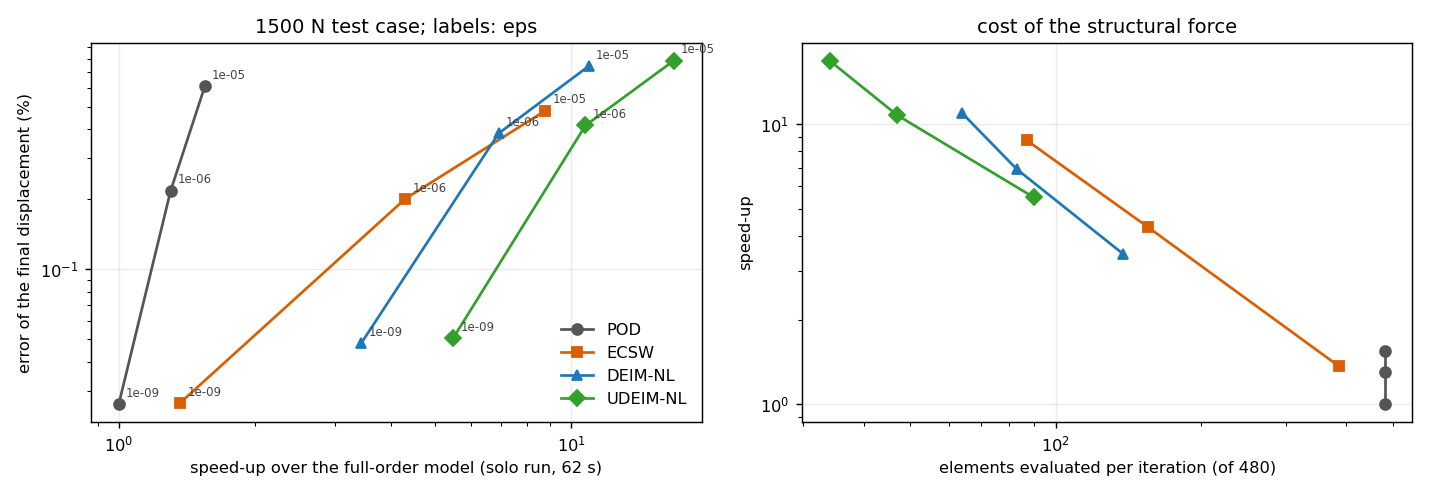
\includegraphics[width=0.85\linewidth]{figures/ch14r/as3_rom_speedup.png}
\caption{3D joint: speed-up of the reduced models.}\label{fig:vf-as3-speed}
\end{figure}

The ECSW speed-up at $10^{-5}$ is $8.8\times$ for 87 of 480 elements, falling to $1.4\times$ at $10^{-9}$, with an offline set-up of 54~s.

\subsection*{Comparison with the publication}

\begin{table}[tbp]
\centering\footnotesize
\caption{Outcome of the reproduction of \citet{nikiema2026assembly}.}\label{tab:vf-as-cmp}
\begin{tabularx}{\linewidth}{@{}>{\raggedright\arraybackslash}p{4.6cm} >{\raggedright\arraybackslash}X >{\raggedright\arraybackslash}p{2.6cm}@{}}
\toprule
Claim & This work & Outcome\\
\midrule
Contact in increment 2 & increment 1 as stated; matched only by changing the geometry & not reproduced as stated\\
DEIM, UDEIM fail with plain Newton; POD, ECSW converge & fail at $10^{-6}$, converge at $10^{-9}$ (2D); fail in 34 of 36 runs (3D) & reproduced, with the $10^{-9}$ exception\\
Mode counts 3 / 11 / 8 & 3 / 10 / 8 & close\\
Error $1.2$--$1.5\,\%$ & $0.94\,\%$ & close\\
Speed-ups 3.4 / 13.8 / 15.8 / 18.4 & 1.4 / 11.3 / 14.8 / 12.8 & lower, same order\\
Domain partitioning saves cost & error $0.29\,\%$, speed-up $\le2.8$ & partly\\
\bottomrule
\end{tabularx}
\end{table}

\subsection*{Where the assembly study departs from the publication}

The publication's geometry is incomplete: with the stated parameters contact begins in the first increment, so the study continues with a variant that is circumstantial. ECSW needed a much smaller tolerance than the stated 0.5. The 3D part is a pipeline and not a reproduction; it uses a regularised contact law, replaces the connectors by springs, covers one parameter (preload) inside the trained range, and the DEIM-NL and UDEIM-NL variants are additions. Not done: other parameters, the publication's full assembly sizes, and an explanation of why DEIM and UDEIM converge at $\varepsilon=10^{-9}$. Each configuration is a single run.

\subsection*{What the reproductions show}\label{sec:vf-repro-summary}

Taken together, the studies show that \fea{} and \rom{} can rebuild nonlinear shell and beam models, train static-condensation, surrogate and contact ROMs on them, integrate those ROMs in time, compute backbones by harmonic balance, identify modal parameters from sparse data, and supply reference fields and frequency-domain ROMs for studies of learned models; and that in several cases the published quantitative claims are recovered within the authors' tolerance. They also show where the reproduced methods reach their limits: a ROM trained on static solves can fail dynamically when in-plane inertia matters or when the training states do not cover the response; a good displacement error can hide a poor contact force; and DEIM-type hyper-reduction can be accurate on training states and wrong a short distance away. They do not show that the packages are faster than other implementations: speed-ups are compared with published numbers only where the publications give them, and the full-order solvers and meshes differ. Where a study could not be reproduced the report says what the publication omits (mesh, damping, thresholds, definition of the error), and those omissions are part of the result.
